
\section{Classical Mechanics}
(such as kinematics, Newton’s laws, work and
energy, oscillatory motion, rotational
motion about a fixed axis, dynamics of
systems of particles, central forces and
celestial mechanics, three-dimensional
particle dynamics, Lagrangian and
Hamiltonian formalism, noninertial
reference frames, elementary topics in
fluid dynamics)



\subsection{Kinematics} 
\Table{
\hline

$v(t) = $ & $v(t) = v_0 + at$

\\ \hline

$x(t) = $ & $x(t) = x_0 + vt + \dfrac{1}{2}at^2$

\\ \hline

\MiniPg{.4}{$v(x)$ in uniform acceleration }

&

\MiniPg{.6}{
\center

$KE = KE_0 + W$

$\dfrac{1}{2}mv^2 = \dfrac{1}{2}m v_0^2 +  ma(x-x_0)$

$v(x) = \sqrt{v_0^2 + 2a(x - x_0)}$

}

\\ \hline

}

%%%%

\Table{
\hline

Projectile motion: $v_{xi} = $ & $v_{xi} = v_i\cos\theta_{i}$

\\ \hline

Projectile motion: $v_{yi} = $ & $v_{yi} = v_i\sin\theta_{i}$

\\ \hline

\MiniPg{.3}{
Acceleration (tangential) of a particle on a fixed track, $y(x)$, in a gravitational field
}

&

\MiniPg{.7}{

Position vector for the track: $\vec f(x) = (x, y(x))$.

Tangential vector: $\vec T(x) = \frac{d \vec f}{dx} = (1, \frac{dy}{dx}). $

Tangential acceleration: $a(x) = \vec g \cdot  \dfrac{\vec T}{|\vec T|}. $ 

Supposing $\vec g$ is in the $y$-direction, $\boxed{a(x) = \dfrac{g\,T_y}{|\vec T|}}.$
}
\\ \hline
}


%===========================================%


\subsection{Newton's Laws, implications, common forces} 

\Table{
\hline

Newton's Law I

&

\MiniPg{.7}{
\center

Law of Inertia: Every body persists in its state of being at rest or of moving uniformly straight forward, except insofar as it is compelled to change its state by force impressed. 
}

\\ \hline
}

%%%%

\Table{
\hline

Newton's Law II

&

\MiniPg{.7}{
\center
Force Law: The alteration of motion is ever proportional to the motive force impress'd; and is made in the direction of the right line in which that force is impress'd.

$\bold{F}_{net} = \dfrac{d \bold{p} }{dt} = m\bold{a}$
}

\\ \hline
}

%%%%

\Table{
\hline
Newton's Law III

&

\MiniPg{.7}{
\center
Action-Reaction Law: To every action there is always opposed an equal reaction: or the mutual actions of two bodies upon each other are always equal, and directed to contrary parts.

$\bold{F}_{12} = - \bold{F}_{21}$
}
\\ \hline
}

%%%%

\Table{
\hline

Law of gravitation: &\MiniPg{.7}{ \center $F_g = G \dfrac{m_1m_2}{r^2}$}

\\ \hline
}

%%%%

\Table{
\hline

\MiniPg{.4}{\center
Force of static friction 
}
&

\MiniPg{.6}{\center
 $f_s \leq \mu_s n$
 }

 \\ \hline

Force of kinetic friction & $f_k = \mu_k n$

\\ \hline

Resistive force at low speed: & $\bold{R} = -b\bold{v}$

\\ \hline

Resistive force at high speed: & $\bold{R} = - c\bold{v}^2$

\\ \hline
}

%%%%

\Table{
\hline

\MiniPg{.4}{
Differential for object falling though resistive medium.
}

&

$\dfrac{dv}{dt} = g - \dfrac{b}{m}v$ 

$v(t) = \dfrac{mg}{b}(1-e^{-bt/m})$ 

\\ \hline

Terminal speed: 

&

\MiniPg{.6}{

\center

 $v_T = \dfrac{mg}{b}$, or $v_T = \sqrt{ \dfrac{mg}{c}}$, or $v_T = \sqrt{ \dfrac{2mg}{D \rho A}}$
}

\\ \hline
}

%%%%%%%%%%%%%%%%%%%%%%%%%%%%%%%%%%%%

\subsection{Work and Energy}

\Table{
\hline

Potential from a given force & $U = -\int_{ref}^{r} \bold{F} \cdot d\bold{r}$

\\ \hline

Force from a given potential & $\bold{F}(x) = -\dfrac{\partial U}{\partial x} \hat x$ \\
& or, rather, $\bold{F}  = - \nabla U$
 
\\ \hline

Work $W = $ & $W = \int_{x_i}^{x_f} \bold{F}_x \cdot d\bold{x} = Fd \cos\theta $

\\ \hline

Kinetic Energy, friction, work & $\Delta KE = -f_k \Delta x + W_{net}$

\\ \hline
}

%%%%

\Table{
\hline

Power: & $P =  \dfrac{dE}{dt} = \dfrac{dW}{dt} = \bold{F} \cdot \bold{v} $

\\ \hline

Average power: & $ \bar{P} = \dfrac{W}{\Delta t}$

\\ \hline

Gravitational potential energy: & $U_g = mgh = - G \dfrac{m_1m_2}{r}$

\\ \hline

Conservation of energy: & $KE + U + E_{internal} = constant$

\\ \hline

Impulse & $\bold{I} = \int_{t_i}^{t_f} \sum \bold{F_{ext}}dt = \Delta \bold{p}_{tot}$

 \\ \hline
}

%%%%%%%%%%%%%%%%%%%%%%%%%%%%%%%%%%%%%%%%%%%%

\subsection{Oscillatory motion}
\Table{
\hline

Hooke's law: & $F_s = -kx$

\\ \hline

$x(t) = $	& $x(t) = A \cos(\omega t + \phi) $ \\ 
		& or $x(t) = c_1 \cos(\omega t) + c_2 \sin(\omega t) $

\\ \hline

Resonant frequency & $\omega =  \sqrt{\dfrac{k}{m}}$

\\ \hline

Period	& $T = 2\pi \sqrt{\dfrac{m}{k}} $

\\ \hline
}

%%%%

\Table{
\hline

\MiniPg{.4}{ \center
$a(x) $
} 
&

\MiniPg{.6}{\center
$a(x) = - \omega^2 x $
}

\\ \hline

Kinetic Energy	& $T = \dfrac{1}{2} k \dot{x}^2 = \dfrac{1}{2} k A^2 \sin^2(\omega t + \phi) $

\\ \hline

Elastic potential & $U_s = \dfrac{1}{2} kx^2 = \dfrac{1}{2} k A^2 \cos^2(\omega t + \phi)  $

\\ \hline

Total energy	& $E = \dfrac{1}{2} k A^2 $

\\ \hline
}

%%%%

\Table{
\hline

\MiniPg{.4}{\center

Effective spring coefficient of multiple springs 
}
&
\MiniPg{.6}{\center
Sum in parallel. Reciprocals sum in series.
}

\\ \hline

\MiniPg{.4}{\center

Reduced mass and resonant frequency of two masses connected by a spring.
}
&
\MiniPg{.6}{\center
$\mu = \dfrac{m_1 m_2}{m_1 + m_2}, \ \ \ \ \ \omega =  \sqrt{\dfrac{k}{\mu}}$
}

\\ \hline
}

%%%%

\Table{
\hline

\MiniPg{.3}{
Solution to the damped harmonic oscillator
}

&

\MiniPg{.7}{
\center
Homogeneous second order D.E.: $m \ddot x + c \dot x + kx = 0 $.

Solution of the form $x(t) = e^{\lambda t}$.

Auxiliary equation: $m \lambda^2 + c \lambda + k = 0 $.

Roots: $\lambda = \dfrac{-c \pm \sqrt{c^2 - 4mk}}{2m}$.

Resulting behavior:

$c^2 - 4mk > 0 \ \  \rightarrow $ Overdamped (Slower exponential decay)

$c^2 - 4mk = 0 \ \ \rightarrow $ Critically damped (Fastest exponential decay)

$c^2 - 4mk < 0  \ \ \rightarrow $ Underdamped (Exp. decaying sinusoid)

}

\\ \hline
}

%%%%

\Table{
\hline

Damping coefficient 

&

\MiniPg{.7}{

If $F_{damping} = -cv $ then the damping coefficient is $ \gamma = \dfrac{c}{2m}$.
}
\\ \hline
}

%%%%

\Table{
\hline

\MiniPg{.3}{
Damping ratio and damping
}

&

\MiniPg{.7}{
\center

Using $\omega_0 = \sqrt{k/m}$, rewrite: $\ddot x + 2 \zeta \omega_0 \dot x + \omega_0^2 x = 0,$ where $\zeta = \dfrac{c}{2\sqrt{mk}}$ is the `damping ratio'.

Solution of the form $x(t) = e^{\lambda t}$.

Auxiliary equation: $\lambda^2 + 2 \zeta \omega_0 \lambda + \omega_0^2 = 0 $.

Roots: $\lambda = \dfrac{- 2 \zeta \omega_0 \pm \sqrt{4\zeta^2\omega_0^4 - 4\omega_0^2}}{2}$.


$ \zeta = \dfrac{c}{2m\omega_0} $ 

$\zeta >1 \ \  \rightarrow $ Overdamped

$\zeta =1 \ \ \rightarrow $ Critically damped 

$\zeta <1 \ \ \rightarrow $ Underdamped
}

\\ \hline
}
 
%%%%

\Table{
\hline
\MiniPg{.3}{
Underdamped oscillator solution
}

&

\MiniPg{.7}{

$x(t) = e^{-\gamma t}a \cos(\omega_1^2 t - \alpha)$, where $\omega_1 = \sqrt{\omega_0^2 - \gamma^2} = \omega_0 \sqrt{1-\zeta^2},$ using $\gamma = \omega_0 \zeta$. This is an exponentially decaying sinusoid. In full glory: $x(t) = e^{-\frac{c}{2m} t}a \cos\BigP{\omega_0^2\BigP{1- \dfrac{c^2}{4mk}} t - \alpha}$.
 
 } 
 \\ \hline
}

%%%%

\Table{
\hline

\MiniPg{.3}{
3 masses and 2 springs,
find modes and frequencies
}

&

\MiniPg{.7}{
\tiny \url{http://scienceworld.wolfram.com/physics/SpringsThreeMasses.html}  
}

\\ \hline
}


%%%%%%%%%%%%%%%%%%%%%%%%%%%%%%%%%%%%%%%%%


\subsection{Rotational motion about a fixed axis}

\Table{
\hline

Centripetal acceleration

&

\MiniPg{.6}{
\center
$a_c = \dfrac{v^2}{r} = \dfrac{(\dfrac{2 \pi r}{T})^2}{r} = \dfrac{4 \pi^2 r}{T^2} = \omega^2 r$

\GraphicWHN{.7}{.37}{CentAccGeomProof.png}
\center \tiny \url{http://hyperphysics.phy-astr.gsu.edu/hbase/cf.html}

}

\\ \hline
}

%%%%

\Table{
\hline

Period: $T = $ & $T = \dfrac{2 \pi r}{v}$

\\ \hline

Tangential acceleration: $a_t = $ & $a_t = \dfrac{d |\bold{v}|}{dt}$

\\ \hline
}

%%%%

\Table{
\hline

Radial acceleration: $a_r = $ & $a_r = -a_c = \dfrac{-v^2}{r}$

\\ \hline

Total acceleration $\bold{a} =$ & $\bold{a_r} + \bold{a_t}$

\\ \hline

}

%%%%

\Table{
\hline
Angular position & $ \theta = \dfrac{s}{r} $

\\ \hline

Angular velocity & $ \omega = \dfrac{d \theta}{dt} = \dfrac{v}{r} $

\\ \hline

Angular acceleration & $ \alpha = \dfrac{d^2 \theta}{dt^2} = \dfrac{a}{r} $

\\ \hline
}

%%%%

\Table{
\hline

Angular position a.a.f.o. time & $\theta(t) = \dfrac{1}{2} \alpha t^2 + \omega t + \theta_0$

\\ \hline

Angular velocity a.a.f.o. time & $\omega(t) = \alpha t + \omega_0$

\\ \hline
}

%%%%

\Table{
\hline
Torque & $\pmb{\tau} = \bold{r} \times \bold{F} = I\alpha $

\\ \hline

Angular momentum 

& 

$\bold{L} = \bold{r} \times \bold{p} \ \ \ \ \ \bold{L}_{body} = I \omega $

\\ \hline
}

%%%%

\Table{
\hline
 
Moment of inertia

&

$I = \sum_i m_i r_i^2 = \int_{0}^{M}r^2 \,dm = \int_{V}r^2 \rho \, dV$ 
 
 \\ \hline
 
 Rotational Kinetic Energy & $ E_{Rot} = \dfrac{1}{2} I \omega^2 = \dfrac{L^2}{2I}$
 
 \\ \hline
}

%%%%

\Table{
\hline
 
 Radius of gyration & $R_g = \sqrt{I/M} $
 
 \\ \hline

 Frequency of pendulum of arbitrary shape & $\omega = \sqrt{\dfrac{MgR_{com}}{I}}$
 
 \\ \hline
}

%%%%

\Table{
\hline

\MiniPg{.3}{
Angular frequency gyroscopic precession
}

&

\MiniPg{.7}{
\center

Consider the old bicycle tire on a string trick. The tire is connected to the string by a rod of length $r$. Consider a change to the tire's angular momentum vector $\bold{L}$ pointing out to the side.

\MPalign{

d\bold{L} &= \pmb{\tau} \, dt \\
dL &= Mgr \, dt \\

}

Also, $dL = L \, d\theta$, and we are interested in $d\theta$, so

\MPalign{

d \theta &= \dfrac{dL}{L} = \dfrac{Mgr}{L}\,dt \\
\omega_{\textrm{precession}} &= \dfrac{Mgr}{L}

}

}

\\ \hline
}

%%%%%

\Table{
\hline

\MiniPg{.3}{

Moment of inertia and frequency of a mass on a massless pendulum of length $l$. 

}

&

\MiniPg{.7}{
\center

$I = ml^2 $ 

$I \vec{\ddot \theta} =  \pmb{\tau} = \bold{r} \times \bold{F}
\ \ \rightarrow \ \ 
I \ddot \theta = -rmg \sin \theta \approx -rmg\theta$ 

Think Hooke's law: $m \ddot x = -kx \rightarrow \omega = \sqrt{\dfrac{k}{m}}$ 

$\boxed{\omega = \sqrt{\dfrac{g}{l}}}$
}

 \\ \hline
}

%%%%

\Table{
\hline

Parallel Axis Theorem & $I_{new} = I_{cm} + md^2$

\\ \hline

\MiniPg{.3}{

Angular frequency of hoop on a nail

}

&

$\sqrt{\dfrac{g}{2r}}$

\\ \hline
}


%%%%%%%%%%%%%%%%%%%%%%%%%%%%%%%%%%%%%%%

\subsection{Dynamics of systems of particles}

\Table{
\hline

Center of mass

&

\MiniPg{.7}{
\center

System of particles: $\Mtx{R} = \dfrac{1}{M} \sum_{i=1}^n m_i \bold{r}_i$

Continuous volume: $\Mtx{R} = \dfrac{1}{M}  \bigint_V \rho(\bold{r}) \bold{r} dV$

}


\\ \hline
}

%%%%

\Table{
\hline

Elastic collision

& 

\MiniPg{.7}{
Total energy and total momentum are both conserved.
}

\\ \hline

\MiniPg{.3}{
Elastic collision with velocities along the x-direction
}

&

\MiniPg{.7}{
$v_{i1} - v_{i2} = v_{f1} - v_{f2}$ ??? is x axis the axis of approach?
}

\\ \hline

\MiniPg{.3}{

Momentum of center of mass in elastic collision

}

&

$MV_{CM,i} = MV_{CM,f}$

\\ \hline
}

%%%%
\Table{
\hline
Inelastic collision 	
&

\MiniPg{.7}{
Kinetic energy is not conserved, but total momentum is. e.g. sticking globs.
}

\\ \hline
}

%%%%


\Table{
\hline
Rocket equation

&

\MiniPg{.7}{
\center

 $m \dfrac{dV}{dt} = -v_e \dfrac{dm}{dt}$ where $m$ is the mass of the rocket, $V$ is the velocity according to an outside observer, and $-v_e$ is the exhaust speed in the rocket frame. Solving this yields
 
$\Delta V = v_e \ln \dfrac{m_0}{m_1}$.

}
\\ \hline
}

%%%%%%%%%%%%%%%%%%%%%%%%%%%%%%%%%%%%%%%%

\subsection{Central forces and celestial mechanics}
\Table{
\hline

\textbf{Kepler's Law I}

& 

\MiniPg{.7}{
\center
The orbit of every planet is an ellipse with the Sun at one of the two foci:

$r(\theta) = \dfrac{p}{1 + \mathcal{E} \cos \theta},$ 

where $\theta = 0$ indicates the direction toward the periapsis.
}

\\ \hline
}

%%%%

\Table{
\hline

peri- vs. apo- & peri- = closest ... apo- = farthest

\\ \hline
}

%%%%

\Table{
\hline

Semi-major axis & Arithmetic mean between $ r_p$ and $ r_a$. \\
			  & $ r_a - a = a -  r_p$ \\
			  & $ a = \dfrac{p}{1- \mathcal{E}^2} $
			  
\\ \hline
}

%%%%

\Table{
\hline

Semi-minor axis & Geometric mean between $ r_p$ and $ r_a$. \\
			  & $ \dfrac{ r_a}{b} = \dfrac{b} { r_p} $\\
			  & $ b = \dfrac{p}{\sqrt{1 - \mathcal{E}^2}} $
			  
\\ \hline
}

%%%%

\Table{
\hline

Semi-latus rectum $p$	& Harmonic mean between $ r_p$ and $ r_a$. \\
					& $ \dfrac{1}{ r_p}  - \dfrac{1}{p} =  \dfrac{1}{p} - \dfrac{1}{ r_a} $ \\
					& $ pa = r_a  r_p = b^2 $

\\ \hline
}

%%%%

\Table{
\hline

Eccentricity calculation	& A.K.A. coefficient of variation between $ r_p$ and $ r_a$. \\
					&  $\mathcal{E} = \dfrac{ r_a -  r_p}{ r_a +  r_p}$
				
\\ \hline
}

%%%%

\Table{
\hline

Eccentricity values 		& $\mathcal{E} = 0 \ \ \  \rightarrow $ circle  \\
					& $ 0 < \mathcal{E} < 1 \ \ \ \rightarrow $ ellipse  \\
					& $\mathcal{E} = 1 \ \ \  \rightarrow $ parabola  \\
					& $\mathcal{E} > 1 \ \ \ \rightarrow $ hyperbola 

\\ \hline
}

%%%%

\Table{
\hline

Area of the elipse 	& $A=\pi a b$

 \\ \hline
}

%%%%

\begin{figure}[htbp]
    \begin{center}
	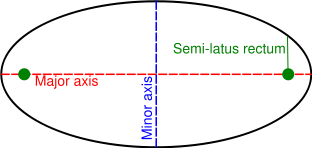
\includegraphics[width=80mm]{images/MajMinSemlatRec.png}
    \end{center}
    \linespread{1} 
	\caption[Ellipse notation]{
	Ellipse notation. When an $r$ for an orbiting object coincides with the semi-latus rectum, $\theta = \pi /2$.
	}
\label{EllipseNotation}
\end{figure}



\Table{
\hline

\textbf{Kepler's Law II} 	& A line joining a planet and the Sun sweeps  \\
					& out equal areas during equal intervals of time. \\
					& $\dfrac{dA}{dt} = \dfrac{1}{2}r^2 \dfrac{d \theta}{dt}$

\\ \hline
}

%%%%

\Table{
\hline

Period				& $P \cdot \dfrac{1}{2} r^2  \dfrac{d \theta}{dt} = \pi a b$

\\ \hline

Mean motion			& $n = 2 \pi / P$ \\
					& $r^2 \ d\theta = abn \ dt$

\\ \hline
}

%%%%

\Table{
\hline

\textbf{Kepler's Law III}

&
\MiniPg{.7}{
\center

The square of the orbital period of a planet is directly proportional to the cube of the semi-major axis of its orbit.

$\dfrac{T^2}{a^3} = \dfrac{4 \pi^2}{G(M + m)}$,

(Importantly) $T^2 \propto a^3 $
}

\\ \hline
}

%%%%

\Table{
\hline

Derive $T$ for circular orbit of & $ \dfrac{GMm}{r^2} = \dfrac{mv^2}{r} = m\omega^2r = \dfrac{mr(2 \pi)^2}{T^2} $ \\
planet about fixed mass $M$. & $T = \sqrt{\dfrac{4 \pi^2 r^3}{G M}}$

\\ \hline
}

%%%%%%%%%%%%%%%%%%%%%%%%%%%%%%%%%%%%%%%%%%%%%%%%%

\subsection{Three-dimensional particle dynamics}

%%%%%%%%%%%%%%%%%%%%%%%%%%%%%%%%%%%%%%%%%%%%%%%%%

\subsection{Lagrangian and Hamiltonian formalism}

\Table{
\hline

Lagrangian &

\MiniPg{.7}{\center $L = L(q,\dot{q},t) = T - V$}

\\ \hline

Euler-Lagrange equation & $\dfrac{\partial{L}}{\partial{q}} = \dfrac{d}{dt}\dfrac{\partial{L}}{\partial{\dot{q}}}$

\\ \hline

Action & $S = \int_{t_0}^{t_1} L(q(t),\dot{q}(t),t)dt$

\\ \hline
}

%%%%

\Table{
\hline

Principal of least action &
\MiniPg{.7}{
The path taken by the system between times $t_0$ and $t_1$ is the one for which the action is stationary (no change) to first order.
 $\delta S = 0$
}
    

\\ \hline

Conjugate momentum & $p = \dfrac{\partial L}{\partial \dot{q}}$

\\ \hline
}

%%%%

\Table{
\hline

Hamiltonian & $H = p\dot{q} - L = T + V$
 
  \\ \hline

\MiniPg{.3}{

Canonical Hamiltonian equations of motion

}
& 
\MiniPg{.7}{
\center
$\dfrac{\partial H}{\partial q} = - \dot{p}, \hspace{1cm} \dfrac{\partial H}{\partial p} = \dot{q}, \hspace{1cm} \dfrac{\partial H}{\partial t} = - \dfrac{\partial L}{\partial t} $
}
 
\\ \hline
}

%%%%%%%%%%%%%%%%%%%%%%%%%%%%%%%%%%%%%%

\subsection{Noninertial reference frames}

\Table{
\hline

Coriolis Force

&

\MiniPg{.7}{
\center
$\bold{F}_{coriolis} = -2m\pmb{\omega} \times (\bold{v}_{in \ rotating \ frame})$

Mnemonic: Coriolis makes it hard \textbf{2 mov} straight. (Steven Byrnes)
}

\\ \hline

Centrifugal Force

&

$ \bold{F}_{centrifugal} = -m\pmb{\omega} \times (\pmb{\omega} \times \pmb{r})$
 
 \\ \hline
}

%%%%%%%%%%%%%%%%%%%%%%%%%%%%%%%%%%%%%%

\subsection{Elementary topics in fluid dynamics}
\Table{
\hline

\MiniPg{.4}{
Bernoulli's Equation for fluid flow (Incompressible, nonviscous, laminar flow)
}

& 

$p + \rho g y + \dfrac{1}{2} \rho v^2 = constant$

\\ \hline

Incompressible flow

&

\MiniPg{.6}{\center

$\nabla \cdot \bold{u} = 0$, where $\bold{u}$ is the flow velocity. For a pipe this infers $\bold{A} \cdot \bold{u}_{\bot} = \textrm{(cross-sectional area)} \times \textrm{(velocity)} = constant$.
}


\\ \hline
}
%%%%

\Table{
\hline

Buoyancy force

&

$B = \rho_{fluid} V_{disp} g$

%\\ \hline
%    
%    Net force on object in fluid
%    
%    &
%    
%    $F_{\textrm{net}} = 

\\ \hline
}


